%% bare_conf.tex
%% V1.3
%% 2007/01/11
%% by Michael Shell
%% See:
%% http://www.michaelshell.org/
%% for current contact information.
%%
%% This is a skeleton file demonstrating the use of IEEEtran.cls
%% (requires IEEEtran.cls version 1.7 or later) with an IEEE conference paper.
%%
%% Support sites:
%% http://www.michaelshell.org/tex/ieeetran/
%% http://www.ctan.org/tex-archive/macros/latex/contrib/IEEEtran/
%% and
%% http://www.ieee.org/

%%*************************************************************************
%% Legal Notice:
%% This code is offered as-is without any warranty either expressed or
%% implied; without even the implied warranty of MERCHANTABILITY or
%% FITNESS FOR A PARTICULAR PURPOSE! 
%% User assumes all risk.
%% In no event shall IEEE or any contributor to this code be liable for
%% any damages or losses, including, but not limited to, incidental,
%% consequential, or any other damages, resulting from the use or misuse
%% of any information contained here.
%%
%% All comments are the opinions of their respective authors and are not
%% necessarily endorsed by the IEEE.
%%
%% This work is distributed under the LaTeX Project Public License (LPPL)
%% ( http://www.latex-project.org/ ) version 1.3, and may be freely used,
%% distributed and modified. A copy of the LPPL, version 1.3, is included
%% in the base LaTeX documentation of all distributions of LaTeX released
%% 2003/12/01 or later.
%% Retain all contribution notices and credits.
%% ** Modified files should be clearly indicated as such, including  **
%% ** renaming them and changing author support contact information. **
%%
%% File list of work: IEEEtran.cls, IEEEtran_HOWTO.pdf, bare_adv.tex,
%%                    bare_conf.tex, bare_jrnl.tex, bare_jrnl_compsoc.tex
%%*************************************************************************

% *** Authors should verify (and, if needed, correct) their LaTeX system  ***
% *** with the testflow diagnostic prior to trusting their LaTeX platform ***
% *** with production work. IEEE's font choices can trigger bugs that do  ***
% *** not appear when using other class files.                            ***
% The testflow support page is at:
% http://www.michaelshell.org/tex/testflow/



% Note that the a4paper option is mainly intended so that authors in
% countries using A4 can easily print to A4 and see how their papers will
% look in print - the typesetting of the document will not typically be
% affected with changes in paper size (but the bottom and side margins will).
% Use the testflow package mentioned above to verify correct handling of
% both paper sizes by the user's LaTeX system.
%
% Also note that the "draftcls" or "draftclsnofoot", not "draft", option
% should be used if it is desired that the figures are to be displayed in
% draft mode.
%
\documentclass[conference]{IEEEtran}
% Add the compsoc option for Computer Society conferences.
%
% If IEEEtran.cls has not been installed into the LaTeX system files,
% manually specify the path to it like:
% \documentclass[conference]{../sty/IEEEtran}





% Some very useful LaTeX packages include:
% (uncomment the ones you want to load)


% *** MISC UTILITY PACKAGES ***
%
%\usepackage{ifpdf}
% Heiko Oberdiek's ifpdf.sty is very useful if you need conditional
% compilation based on whether the output is pdf or dvi.
% usage:
% \ifpdf
%   % pdf code
% \else
%   % dvi code
% \fi
% The latest version of ifpdf.sty can be obtained from:
% http://www.ctan.org/tex-archive/macros/latex/contrib/oberdiek/
% Also, note that IEEEtran.cls V1.7 and later provides a builtin
% \ifCLASSINFOpdf conditional that works the same way.
% When switching from latex to pdflatex and vice-versa, the compiler may
% have to be run twice to clear warning/error messages.






% *** CITATION PACKAGES ***
%
\usepackage{cite}
% cite.sty was written by Donald Arseneau
% V1.6 and later of IEEEtran pre-defines the format of the cite.sty package
% \cite{} output to follow that of IEEE. Loading the cite package will
% result in citation numbers being automatically sorted and properly
% "compressed/ranged". e.g., [1], [9], [2], [7], [5], [6] without using
% cite.sty will become [1], [2], [5]--[7], [9] using cite.sty. cite.sty's
% \cite will automatically add leading space, if needed. Use cite.sty's
% noadjust option (cite.sty V3.8 and later) if you want to turn this off.
% cite.sty is already installed on most LaTeX systems. Be sure and use
% version 4.0 (2003-05-27) and later if using hyperref.sty. cite.sty does
% not currently provide for hyperlinked citations.
% The latest version can be obtained at:
% http://www.ctan.org/tex-archive/macros/latex/contrib/cite/
% The documentation is contained in the cite.sty file itself.


% Meto paquetes a huevo
\usepackage{graphicx}
\usepackage[table]{xcolor}

% *** GRAPHICS RELATED PACKAGES ***
%
%\ifCLASSINFOpdf
  % \usepackage[pdftex]{graphicx}
  % declare the path(s) where your graphic files are
  % \graphicspath{{../pdf/}{../jpeg/}}
  % and their extensions so you won't have to specify these with
  % every instance of \includegraphics
  % \DeclareGraphicsExtensions{.pdf,.jpeg,.png}
%\else
  % or other class option (dvipsone, dvipdf, if not using dvips). graphicx
  % will default to the driver specified in the system graphics.cfg if no
  % driver is specified.
  % \usepackage[dvips]{graphicx}
  % declare the path(s) where your graphic files are
  % \graphicspath{{../eps/}}
  % and their extensions so you won't have to specify these with
  % every instance of \includegraphics
  % \DeclareGraphicsExtensions{.eps}
%\fi
% graphicx was written by David Carlisle and Sebastian Rahtz. It is
% required if you want graphics, photos, etc. graphicx.sty is already
% installed on most LaTeX systems. The latest version and documentation can
% be obtained at: 
% http://www.ctan.org/tex-archive/macros/latex/required/graphics/
% Another good source of documentation is "Using Imported Graphics in
% LaTeX2e" by Keith Reckdahl which can be found as epslatex.ps or
% epslatex.pdf at: http://www.ctan.org/tex-archive/info/
%
% latex, and pdflatex in dvi mode, support graphics in encapsulated
% postscript (.eps) format. pdflatex in pdf mode supports graphics
% in .pdf, .jpeg, .png and .mps (metapost) formats. Users should ensure
% that all non-photo figures use a vector format (.eps, .pdf, .mps) and
% not a bitmapped formats (.jpeg, .png). IEEE frowns on bitmapped formats
% which can result in "jaggedy"/blurry rendering of lines and letters as
% well as large increases in file sizes.
%
% You can find documentation about the pdfTeX application at:
% http://www.tug.org/applications/pdftex





% *** MATH PACKAGES ***
%
\usepackage[cmex10]{amsmath}
% A popular package from the American Mathematical Society that provides
% many useful and powerful commands for dealing with mathematics. If using
% it, be sure to load this package with the cmex10 option to ensure that
% only type 1 fonts will utilized at all point sizes. Without this option,
% it is possible that some math symbols, particularly those within
% footnotes, will be rendered in bitmap form which will result in a
% document that can not be IEEE Xplore compliant!
%
% Also, note that the amsmath package sets \interdisplaylinepenalty to 10000
% thus preventing page breaks from occurring within multiline equations. Use:
%\interdisplaylinepenalty=2500
% after loading amsmath to restore such page breaks as IEEEtran.cls normally
% does. amsmath.sty is already installed on most LaTeX systems. The latest
% version and documentation can be obtained at:
% http://www.ctan.org/tex-archive/macros/latex/required/amslatex/math/





% *** SPECIALIZED LIST PACKAGES ***
%
%\usepackage{algorithmic}
% algorithmic.sty was written by Peter Williams and Rogerio Brito.
% This package provides an algorithmic environment fo describing algorithms.
% You can use the algorithmic environment in-text or within a figure
% environment to provide for a floating algorithm. Do NOT use the algorithm
% floating environment provided by algorithm.sty (by the same authors) or
% algorithm2e.sty (by Christophe Fiorio) as IEEE does not use dedicated
% algorithm float types and packages that provide these will not provide
% correct IEEE style captions. The latest version and documentation of
% algorithmic.sty can be obtained at:
% http://www.ctan.org/tex-archive/macros/latex/contrib/algorithms/
% There is also a support site at:
% http://algorithms.berlios.de/index.html
% Also of interest may be the (relatively newer and more customizable)
% algorithmicx.sty package by Szasz Janos:
% http://www.ctan.org/tex-archive/macros/latex/contrib/algorithmicx/




% *** ALIGNMENT PACKAGES ***
%
%\usepackage{array}
% Frank Mittelbach's and David Carlisle's array.sty patches and improves
% the standard LaTeX2e array and tabular environments to provide better
% appearance and additional user controls. As the default LaTeX2e table
% generation code is lacking to the point of almost being broken with
% respect to the quality of the end results, all users are strongly
% advised to use an enhanced (at the very least that provided by array.sty)
% set of table tools. array.sty is already installed on most systems. The
% latest version and documentation can be obtained at:
% http://www.ctan.org/tex-archive/macros/latex/required/tools/


%\usepackage{mdwmath}
%\usepackage{mdwtab}
% Also highly recommended is Mark Wooding's extremely powerful MDW tools,
% especially mdwmath.sty and mdwtab.sty which are used to format equations
% and tables, respectively. The MDWtools set is already installed on most
% LaTeX systems. The lastest version and documentation is available at:
% http://www.ctan.org/tex-archive/macros/latex/contrib/mdwtools/


% IEEEtran contains the IEEEeqnarray family of commands that can be used to
% generate multiline equations as well as matrices, tables, etc., of high
% quality.


%\usepackage{eqparbox}
% Also of notable interest is Scott Pakin's eqparbox package for creating
% (automatically sized) equal width boxes - aka "natural width parboxes".
% Available at:
% http://www.ctan.org/tex-archive/macros/latex/contrib/eqparbox/





% *** SUBFIGURE PACKAGES ***
%\usepackage[tight,footnotesize]{subfigure}
% subfigure.sty was written by Steven Douglas Cochran. This package makes it
% easy to put subfigures in your figures. e.g., "Figure 1a and 1b". For IEEE
% work, it is a good idea to load it with the tight package option to reduce
% the amount of white space around the subfigures. subfigure.sty is already
% installed on most LaTeX systems. The latest version and documentation can
% be obtained at:
% http://www.ctan.org/tex-archive/obsolete/macros/latex/contrib/subfigure/
% subfigure.sty has been superceeded by subfig.sty.



%\usepackage[caption=false]{caption}
%\usepackage[font=footnotesize]{subfig}
% subfig.sty, also written by Steven Douglas Cochran, is the modern
% replacement for subfigure.sty. However, subfig.sty requires and
% automatically loads Axel Sommerfeldt's caption.sty which will override
% IEEEtran.cls handling of captions and this will result in nonIEEE style
% figure/table captions. To prevent this problem, be sure and preload
% caption.sty with its "caption=false" package option. This is will preserve
% IEEEtran.cls handing of captions. Version 1.3 (2005/06/28) and later 
% (recommended due to many improvements over 1.2) of subfig.sty supports
% the caption=false option directly:
%\usepackage[caption=false,font=footnotesize]{subfig}
%
% The latest version and documentation can be obtained at:
% http://www.ctan.org/tex-archive/macros/latex/contrib/subfig/
% The latest version and documentation of caption.sty can be obtained at:
% http://www.ctan.org/tex-archive/macros/latex/contrib/caption/




% *** FLOAT PACKAGES ***
%
%\usepackage{fixltx2e}
% fixltx2e, the successor to the earlier fix2col.sty, was written by
% Frank Mittelbach and David Carlisle. This package corrects a few problems
% in the LaTeX2e kernel, the most notable of which is that in current
% LaTeX2e releases, the ordering of single and double column floats is not
% guaranteed to be preserved. Thus, an unpatched LaTeX2e can allow a
% single column figure to be placed prior to an earlier double column
% figure. The latest version and documentation can be found at:
% http://www.ctan.org/tex-archive/macros/latex/base/


\usepackage{subfig}
%\usepackage{stfloats}
% stfloats.sty was written by Sigitas Tolusis. This package gives LaTeX2e
% the ability to do double column floats at the bottom of the page as well
% as the top. (e.g., "\begin{figure*}[!b]" is not normally possible in
% LaTeX2e). It also provides a command:
%\fnbelowfloat
% to enable the placement of footnotes below bottom floats (the standard
% LaTeX2e kernel puts them above bottom floats). This is an invasive package
% which rewrites many portions of the LaTeX2e float routines. It may not work
% with other packages that modify the LaTeX2e float routines. The latest
% version and documentation can be obtained at:
% http://www.ctan.org/tex-archive/macros/latex/contrib/sttools/
% Documentation is contained in the stfloats.sty comments as well as in the
% presfull.pdf file. Do not use the stfloats baselinefloat ability as IEEE
% does not allow \baselineskip to stretch. Authors submitting work to the
% IEEE should note that IEEE rarely uses double column equations and
% that authors should try to avoid such use. Do not be tempted to use the
% cuted.sty or midfloat.sty packages (also by Sigitas Tolusis) as IEEE does
% not format its papers in such ways.





% *** PDF, URL AND HYPERLINK PACKAGES ***
%
\usepackage{url}
% url.sty was written by Donald Arseneau. It provides better support for
% handling and breaking URLs. url.sty is already installed on most LaTeX
% systems. The latest version can be obtained at:
% http://www.ctan.org/tex-archive/macros/latex/contrib/misc/
% Read the url.sty source comments for usage information. Basically,
% \url{my_url_here}.





% *** Do not adjust lengths that control margins, column widths, etc. ***
% *** Do not use packages that alter fonts (such as pslatex).         ***
% There should be no need to do such things with IEEEtran.cls V1.6 and later.
% (Unless specifically asked to do so by the journal or conference you plan
% to submit to, of course. )


% correct bad hyphenation here
\hyphenation{op-tical net-works semi-conduc-tor}

% lindo
\newcommand{\refp}[1]{(\ref{#1})}

\begin{document}
%
% paper title
% can use linebreaks \\ within to get better formatting as desired
\title{\Huge \bf \sc
Design and implementation of sensor fusion and control for an autonomous quadrotor}


% author names and affiliations
% use a multiple column layout for up to three different
% affiliations
\author{\IEEEauthorblockN{Santiago Paternain}
\IEEEauthorblockA{Facultad de Ingeniería\\
Universidad de la República\\
Montevideo, Uruguay\\
spaternain@gmail.com}
\and
\IEEEauthorblockN{Rodrigo Rosa}
\IEEEauthorblockA{Facultad de Ingeniería\\
Universidad de la República\\
Montevideo, Uruguay\\
rodrigorosa.LG@gmail.com}
\and
\IEEEauthorblockN{Mat\'ias Tailani\'an}
\IEEEauthorblockA{Facultad de Ingeniería\\
Universidad de la República\\
Montevideo, Uruguay\\
matias@tailanian.com}
\and
\IEEEauthorblockN{Rafael Canetti}
\IEEEauthorblockA{Facultad de Ingeniería\\
Universidad de la República\\
Montevideo, Uruguay\\
canetti@fing.edu.uy}
}

% conference papers do not typically use \thanks and this command
% is locked out in conference mode. If really needed, such as for
% the acknowledgment of grants, issue a \IEEEoverridecommandlockouts
% after \documentclass

% for over three affiliations, or if they all won't fit within the width
% of the page, use this alternative format:
% 
%\author{\IEEEauthorblockN{Michael Shell\IEEEauthorrefmark{1},
%Homer Simpson\IEEEauthorrefmark{2},
%James Kirk\IEEEauthorrefmark{3}, 
%Montgomery Scott\IEEEauthorrefmark{3} and
%Eldon Tyrell\IEEEauthorrefmark{4}}
%\IEEEauthorblockA{\IEEEauthorrefmark{1}School of Electrical and Computer Engineering\\
%Georgia Institute of Technology,
%Atlanta, Georgia 30332--0250\\ Email: see http://www.michaelshell.org/contact.html}
%\IEEEauthorblockA{\IEEEauthorrefmark{2}Twentieth Century Fox, Springfield, USA\\
%Email: homer@thesimpsons.com}
%\IEEEauthorblockA{\IEEEauthorrefmark{3}Starfleet Academy, San Francisco, California 96678-2391\\
%Telephone: (800) 555--1212, Fax: (888) 555--1212}
%\IEEEauthorblockA{\IEEEauthorrefmark{4}Tyrell Inc., 123 Replicant Street, Los Angeles, California 90210--4321}}




% use for special paper notices
%\IEEEspecialpapernotice{(Invited Paper)}




% make the title area
\maketitle


\begin{abstract}
%\boldmath
This paper describes the design and integration of an instrumentation and control system that allows the autonomous flight of a quadrotor. A comercial frame is acquired, a mathematical model for the quadrotor is developed and its parameters determined from the characterization of the unit. An external intelligence is integrated to play the role of the flight controller. A 9 degrees of freedom Inertial Measurement Unit (IMU) equipped with a barometer is calibrated and added to the platform. Data from the IMU is combined with the information provided by a GPS within a Extended Kalman Filter (EKF) to obtain a reliable estimation of the state variables. The control actions are obtained from a proportional-integral controller based on the LQR algorithm. As shown in section \refp{sec:results-tests}, a stable autonomous platform is achieved.%For windless environments, a stable platform is achieved.
% -cambio-
\end{abstract}
% IEEEtran.cls defaults to using nonbold math in the Abstract.
% This preserves the distinction between vectors and scalars. However,
% if the conference you are submitting to favors bold math in the abstract,
% then you can use LaTeX's standard command \boldmath at the very start
% of the abstract to achieve this. Many IEEE journals/conferences frown on
% math in the abstract anyway.

% no keywords




% For peer review papers, you can put extra information on the cover
% page as needed:
% \ifCLASSOPTIONpeerreview
% \begin{center} \bfseries EDICS Category: 3-BBND \end{center}
% \fi
%
% For peerreview papers, this IEEEtran command inserts a page break and
% creates the second title. It will be ignored for other modes.
\IEEEpeerreviewmaketitle



\section{Introduction}
% no \IEEEPARstart

A quadrotor platform can be imagined performing countless tasks, such as search and rescue, wild fire suppression, or scientific research\cite{bib:apps}. Many applications are being developed based on such platforms, but how do they fly? An aerial vehicle is inherently unstable, staying still is not a simple task. This paper focuses on the stabilization of a quadrotor, explaining the development of the mathematical model \cite{bib:quadrotor-bible}\cite{bib:curso_quad} to represent the system, the filtering techniques applied for sensor data fusion\cite{bib:kalman}\cite{bib:kalman2} and the control system\cite{bib:quadrotor-bible}\cite{bib:lqrnotes} that allows the quadrotor to fly.
% -cambio-
The platform is based on the commercial radio controlled quadrotor, shown in figure \refp{fig:commercial_quadrotor}. The length between opposite propelers is $61.5\;cm$, the wheight is $990\;g$, and it has $1300\;g$ of payload. The frame and the electronic speed controllers (ESCs) used for the motores were preserved, whereas the IMU and intelligence were replaced by the flight controller that was developed. A BeagleBoard\footnote{BeagleBoard development board - \url{http://beagleboard.org/}} running Linux\footnote{Angstrom distribution: \url{http://www.angstrom-distribution.org/}} performs the computations requiered to convert raw data received from the IMU\footnote{\textit{Mongoose} IMU - \url{http://store.ckdevices.com/}} over a UART and combine it using an EKF. The EKF overcomes the problems inherent to each sensor and filters out noise, providing a reliable estimation of the state vector. Once the current state is known, the LQR algorithm\cite{bib:lqrnotes}\cite{bib:lqr-discreto} is used to derive the control actions required to bring the system to the desired setpoint.
% -cambio-
\begin{figure}[h!]
	\centering
	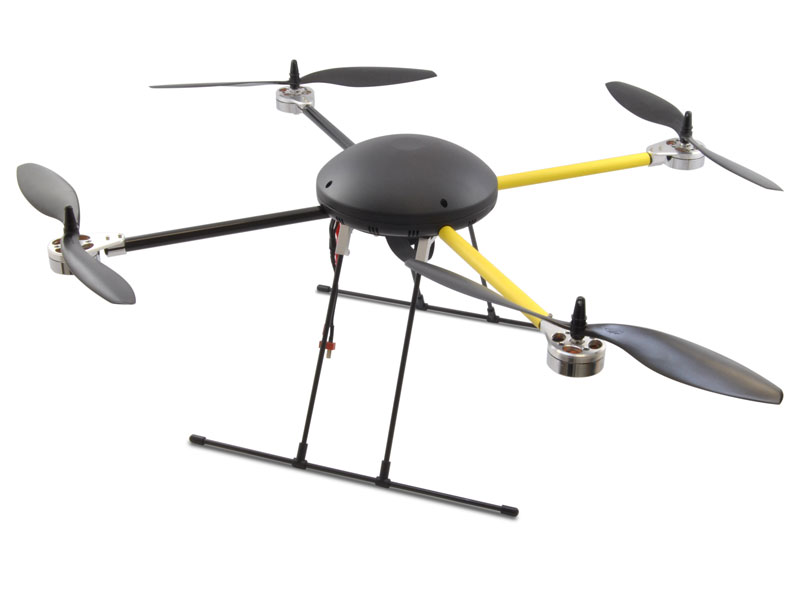
\includegraphics[width=.6\columnwidth]{./pics_paper/foto_quad.jpg}
	\caption{\textbf{Commercial quadrotor acquired.}}
	\label{fig:commercial_quadrotor}
\end{figure}

% You must have at least 2 lines in the paragraph with the drop letter
% (should never be an issue)
%I wish you the best of success.

%\hfill mds
 
%\hfill January 11, 2007
The two main goals are to integrate additional sensors and intelligence to the available platform to obtain a state estimation, and design and integrate a control system that using the state estimation achieves the autonomous flight.
\section{Model of a quadrotor}
\label{sec:modelo}

\subsection{Definitions}
\label{sec:modelo-defs}

A diagram of the quadrotor is shown in figure \refp{fig:quad}. Two of the motors rotate clockwise (2 and 4) and the other two (1 and 3) rotate counterclockwise. This configuration allows the quadrotor to rotate, tilt and gain/lose altitud by setting different speeds on each motor. Two frames of reference (figure \refp{fig:quad}) are constantly used through out this paper: an intertial frame $S_I - \lbrace \hat{i},\hat{j},\hat{k}\rbrace$ ($\lbrace \vec{x},\vec{y},\vec{z}\rbrace$), relative to the Earth, mapped to  North, West and Up respectively, and a non-intertial frame $S_q - \lbrace \hat{i}_q,\hat{j}_q,\hat{k}_q\rbrace$ ($\lbrace \vec{x}_q,\vec{y}_q,\vec{z}_q\rbrace$) relative to the quadrotor. The mapping of one frame to the other can be achieved by applying the three rotations shown in figure \refp{fig:rotaciones}. The angles $\lbrace \theta, \varphi, \psi\rbrace$ are known as Euler angles.

\begin{figure}[h!]
	\centering
	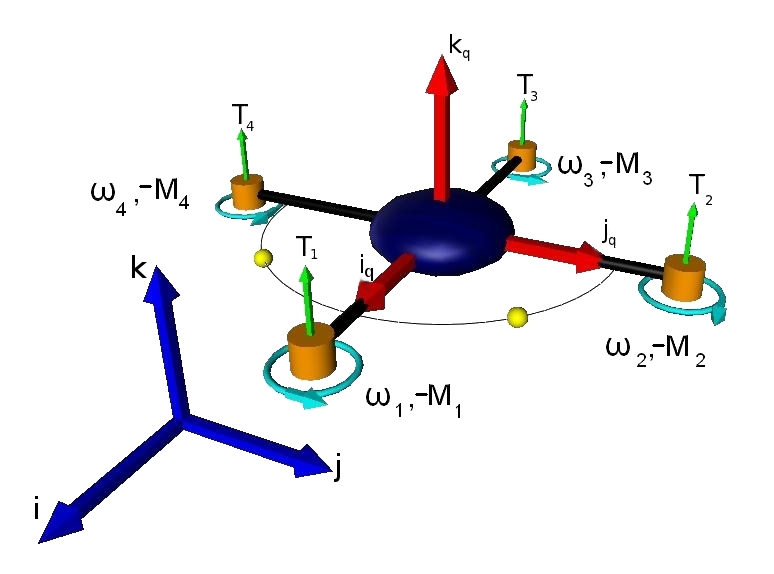
\includegraphics[width=.7\columnwidth]{./pics_paper/quad_coord.jpg}
	\vspace{-5pt}
	\caption{\textbf{Model of the quadrotor -} The blue arrows represent the intertial reference frame $S_I$, and the red arrows represent the non-inertial reference frame $S_q$. The cyan ``looped'' arrows indicate the direction of rotation of each motor, which rotate at $\omega_i$ and generate a torque $M_i$ opposite to their direction of rotation. The arrows labeled $T_{[1,2,3,4]}$ represent the thrust of the motors. The semicircle and the two yellow spheres indicate the $x_q$ axis of the unit.}
    \vspace{-10pt}
	\label{fig:quad}
\end{figure}
\subsection{Dynamics-kinematics of the system}
\label{sec:modelo-dyn-kin}

From a detailed analysis of the dynamics and kinematics of the quadrotor, the equations \refp{eq:modelo} are obtained, and the state vector shown in \refp{eq:sv} is built to describe the system at any given time. The variables with subscript \textit{q} are referenced to the quadrotor frame $S_q$, the rest are relative to $S_I$. This choice simplifies the theoretical development and the interpretation of the data provided by the IMU, which is mounted on the quadrotor and hence provides provides accelerations and angular velocities that are relative to $S_q$:
\begin{equation}
\vec{X}=\left\lbrace  x,y,z, \theta,\varphi,\psi, v_{q_z},v_{q_y},v_{q_z},\omega_{q_x},\omega_{q_y},\omega_{q_z} \right\rbrace
\label{eq:sv}
\end{equation}
where:
\begin{itemize}
\item $\lbrace x,y,z \rbrace$ represent the position of the center of mass of the system in $S_I$.
\item $\lbrace\theta,\varphi,\psi\rbrace$ are the Euler angles shown in figure \refp{fig:rotaciones}.
\item $\lbrace v_{q_x},v_{q_y},v_{q_z}\rbrace$ are the linear velocities relative to $S_q$.
\item $\lbrace w_{q_x},w_{q_y},w_{q_z}\rbrace$ are the angular velocities relative to $S_q$ (right hand rule applied on $\lbrace \hat{i}_q,\hat{j}_q,\hat{k}_q\rbrace$).
\end{itemize}
\vspace{10pt}
\begin{equation}
\small
\boxed{\begin{aligned}&\dot{x}\!=\!v_{q_x} \cos \varphi \cos \theta \!+\! v_{q_y} ( \cos \theta \sin \varphi \sin \psi\!-\!\cos \varphi \sin \theta )\\
&\quad \!+\! v_{q_z}(\sin \psi \sin \theta \!+\! \cos \psi \cos \theta \sin \varphi)\\
&\dot{y}\!=\!v_{q_x} \cos \varphi \sin \theta \!+\! v_{q_y} (\cos \psi \cos \theta \!+\! \sin \theta \sin \varphi \sin \psi)\\
&\quad\!+\! v_{q_z}( \cos \psi \sin \theta \sin \varphi\!-\!\cos \theta \sin \psi )\\
&\dot{z}\!=\! \!-\!v_{q_x} \sin \varphi  \!+\! v_{q_y} \cos \varphi \sin \psi  \!+\! v_{q_z}\cos \varphi \cos \psi\\
&\dot{\psi}\!=\!\omega_{q_x} \!+\! \omega_{q_z}\tan\varphi \cos\psi \!+\! \omega_{q_y}\tan\varphi \sin\psi\\
&\dot{\varphi}\!=\!\omega_{q_y}\cos \psi \!-\! \omega_{q_z}\sin\psi\\
&\dot{\theta}\!=\!\omega_{q_z} \frac{\cos\psi}{\cos\varphi}  \!+\! \omega_{q_y}\frac{\sin\psi}{\cos\varphi}\\
&\dot{v_{q_x}}\!=\!v_{q_y} \omega_{q_z} \!-\! v_{q_z} \omega_{q_y}\!+\!g\sin\varphi\\
&\dot{v_{q_y}}\!=\!v_{q_z} \omega_{q_x} \!-\! v_{q_x} \omega_{q_z}\!-\!g\cos\varphi\sin\psi\\
&\dot{v_{q_z}}\!=\!v_{q_x} \omega_{q_y} \!-\! v_{q_y} \omega_{q_x}\!-\!g\cos\varphi\cos\psi\!+\!\frac{1}{M}\sum_{i\!=\!1}^4T_i\\
&\dot{\omega_{q_x}}\!=\!\frac{1}{I_{xx}}\omega_{q_y}\omega_{q_z}(I_{yy}\!-\!I_{zz})\\
&\quad\!+\!\frac{1}{I_{xx}}\omega_{q_y}I_{zz_m}(\omega_1\!-\!\omega_2\!+\!\omega_3\!-\!\omega_4)\\
&\quad\!-\!\frac{1}{I_{xx}}dMg\cos\varphi\sin\psi\!+\!\frac{1}{I_{xx}}L(T_2\!-\!T_4)\\
&\dot{\omega_{q_y}}\!=\!\frac{1}{I_{yy}}\omega_{q_x}\omega_{q_z}(\!-\!I_{xx}\!+\!I_{zz})\\
&\quad\!+\!\frac{1}{I_{yy}}\omega_{q_x}I_{zz_m}(\omega_1\!-\!\omega_2\!+\!\omega_3\!-\!\omega_4)\\
&\quad\!-\!\frac{1}{I_{yy}}dMg\sin\varphi\!+\!\frac{1}{I_{yy}}L(T_3\!-\!T_1)\\
&\dot{\omega_{q_z}}\!=\!\frac{1}{I_{zz}}\left(\!-\!Q_1\!+\!Q_2\!-\!Q_3\!+\!Q_4\right)\\
%\frac{\!-\!I_{zz_m}(\dot{w_1}\!-\!\dot{w_2}\+!\!\dot{w_3}\!-\!\dot{w_4})}{I_{zz}}\!+\!
\end{aligned}}
\label{eq:modelo}
\end{equation}

\begin{figure}[h!]
  \centering
  \subfloat[Rotation 1: Axis $\hat{k}$]{\label{fig:angulos_1}
  		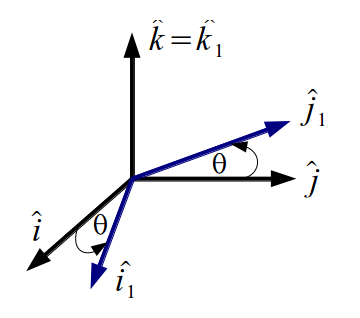
\includegraphics[width=0.3\columnwidth]
  			{../pics_modelo_fisico/angulos_1.png}}
  \subfloat[Rotation 2: Axis $\hat{j}$]{\label{fig:angulos_2} 
  		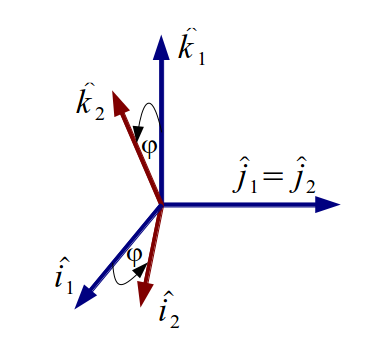
\includegraphics[width=0.3\columnwidth]
  			{../pics_modelo_fisico/angulos_2.png}}
  \subfloat[Rotation 3: Axis $\hat{i}$]{\label{fig:angulos_3} 
  		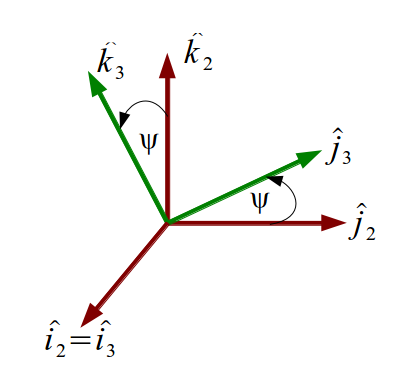
\includegraphics[width=0.3\columnwidth]
  			{../pics_modelo_fisico/angulos_3.png}}
  \caption{\textbf{Mapping -} Rotations applied on $S_I$ to obtain $S_q$.}
  \label{fig:rotaciones}
\end{figure}

\section{Sensors}

In order to determine what actions should be taken, the state of the system must be known. The system uses a 9 degrees of freedom IMU and a GPS. This equipment enables direct measurement of most of the state variables. There is no direct measurement of the linear speed of the system $\{v_{q_z},v_{q_y},v_{q_z}\}$, so the model developed in \refp{sec:modelo} is used to estimate them.

\subsection{IMU}
\label{sec:sensors-imu}

The IMU is equiped with the following sensors:
\begin{itemize}
\item \textbf{Barometer:} Measures the absolute pressure of the environment. Variations of pressure are used to estimate variations in the altitud of the system.
\item \textbf{Thermometer:} The barometer includes a thermometer. The temperature data is used to apply a temperature compensation to the calibrations performed on the gyroscope and the accelerometer.
\item \textbf{Gyroscope:} A 3-axis gyroscope is used to measure angular velocity of $S_q$. A calibration, based on \cite{bib:calib_imu}, was designed and applied to this device, as well as a temperature-compensation.
\item \textbf{Accelerometer:} A 3-axis accelerometer is used to measure gravity. Under the hypothesis that no other accelerations are present, this allows the determination of two of the three Euler angles: $\{\psi, \phi\}$. This hypothesis is acceptable, since the accelerations involved are not significant compared to gravity. A calibration, based on \cite{bib:calib_imu}, was designed and applied to this device, as well as a temperature-compensation.
\item \textbf{Magnetometer:} In an area free of magnetic interference this 3-axis sensor will measure $\vec{B}$, the Earth's magnetic field, allowing to determine what direction is North. If the system is horizontal (or the inclination is estimated using other sensors) this sensor can be used to determine the last of the three Euler angles: $\theta$. A calibration based on \cite{bib:bola} and \cite{bib:alain} was performed on this sensor.
\end{itemize}

The equations used to determine the three Euler angles are the following:
  \[
  \phi = -\arcsin\left(\frac{Acc_x}{\vert\vert\vec{Acc}\vert\vert}\right)
  \]

  \[
  \psi =- \arctan \left(\frac{Acc_y}{Acc_z}\right)
  \]
      
  \[
  \hspace{-20pt}
  M = 
\left(\begin{array}{ccc} \cos\!\left(\mathrm{\phi}\right) & \sin\!\left(\mathrm{\phi}\right)\, \sin\!\left(\mathrm{\psi}\right) & \cos\!\left(\mathrm{\psi}\right)\, \sin\!\left(\mathrm{\phi}\right)\\ 0 & \cos\!\left(\mathrm{\psi}\right) & - \sin\!\left(\mathrm{\psi}\right)\\ - \sin\!\left(\mathrm{\phi}\right) & \cos\!\left(\mathrm{\phi}\right)\, \sin\!\left(\mathrm{\psi}\right) & \cos\!\left(\mathrm{\phi}\right)\, \cos\!\left(\mathrm{\psi}\right) \end{array}\right)
  \]

  \[
  \vec{v} = M . \frac{\vec{B}}{\vert \vert \vec{B} \vert \vert}
  \]

  \[
  \theta = -atan2\left( \frac{v[1]}{v[0]}\right)
  \]



\subsection{GPS}
\label{sec:sensors-gps}

In theory, given some initial position $\{x_0 ,y_0\}$ the accelerometer could be used to determine variations $\{x_0+\Delta x,y_0+\Delta y\}$. In practice this estimation drifts rapidly (tens of meters in a couple of seconds), so a GPS is used to determine the absolute position $\{x,y\}$ of the system, correcting the drift. The accuracy, with good sky visibility, is of 2-3 meters. The GPS's performance improves when the system is moving.

\subsection{Sensor Specifications}
\label{sec:sensors-specifications}

Table \refp{tab:sensors:resumen} shows an outline of the specifications of the sensors used.

\begin{table}[h]
\begin{center}
\rowcolors{1}{gray!20}{}
\begin{tabular}{|c|c|c|}
\hline
 & Rate & Resolution \\
\hline
Accelerometer XY & 10ms (x2)& 4mg\\
\hline
Accelerometer Z  & 10ms (x2)& 4mg\\
\hline
Gyro XY  & 10ms (x2)& 0.07 $^o/s$\\
\hline
Gyro Z  & 10ms (x2)& 0.07 $^o/s$\\
\hline
Barometer  & 10ms (x1) & 1Pa\\
\hline
Magnetometer XY  & 10ms  (x2)& 5 mGa\\
\hline
Magnetometer Z  & 10ms (x2)& 5 mGa\\
\hline
GPS  & 1s & - \\
\hline
\end{tabular}
\end{center}
\caption{\textbf{Sensor specifications:} A rate of ``\textit{10ms (x2)}'' means that every 10ms the result of averaging 2 samples is received from the IMU.}
\label{tab:sensors:resumen}
\end{table}

\section{Kalman Filter}

In order to perform adequate control actions, a reliable estimation of the state variables must be available in real time. The Kalman Filter uses the mathematical model for the system to predict what should happen next given the current state, and corrects the prediction with the information read from the sensors, taking into consideration how much confidence is placed on the prediction and how much on the measurements. This weighted prediction-correction technique allows a smooth state estimation without the typical delay introduced by filtering, even small delays can severly affect the performance of the system.

Every sensor has its issues: The gyro drifts over time; the accelerometer is very sensible to the vibrations generated by the motors; the magnetometer is distorted by ferromagnetic materials; the GPS has a very poor accuracy and a slow update rate. Each sensor by itself is very limited, but they can be combined to compensate for their limitations. The filter takes care of this.

%TODO pasar figura a ingl\'e
\begin{figure}
	\centering
	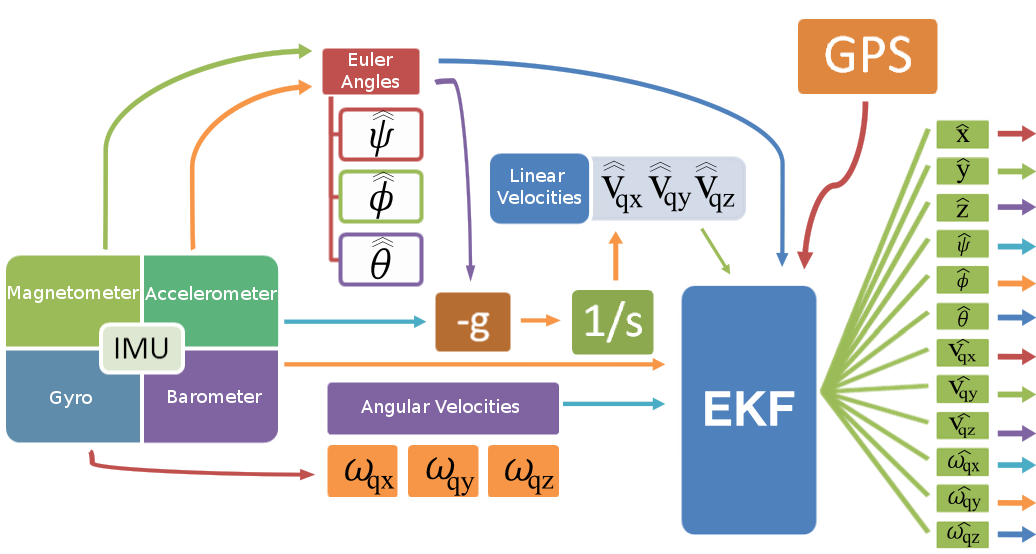
\includegraphics[width=1\columnwidth]{./pics_paper/diagrama_kalman_eng.png}
	\caption{\textbf{EKF - } Outline of how sensor data is combined to estimate the state variables.}
	\label{fig:diagrama_kalman}
\end{figure}

\subsection{EKF}
\label{sec:kalman-ekf}

The theory behind a standard Kalman Filter does not hold for a system that is not linear. The model for the quadrotor given by \refp{eq:modelo} is highly non-linear, so an EKF is implemented based on \cite{bib:kalman} and \cite{bib:kalman2}. An EKF is compatible with non-linear systems, but it is not optimal, the performance is highly dependant on the linearizacion \cite{bib:kay}. The implementation of the EKF gave very good results, and proved to play a critical part in the system. As an example, the data provided by the accelerometer is ``unusable'' without filtering, and experiments with a simple low pass filter (LPF) showed that a 60ms delay introduced by the LPF severly deteriorated the performance of the system. When the EKF was assigned the task of reducing noise, the perfomance was significatively improved.

\subsection{Integration with the system}
\label{sec:kalman-integration}

% \begin{figure}
% 	\centering
% 	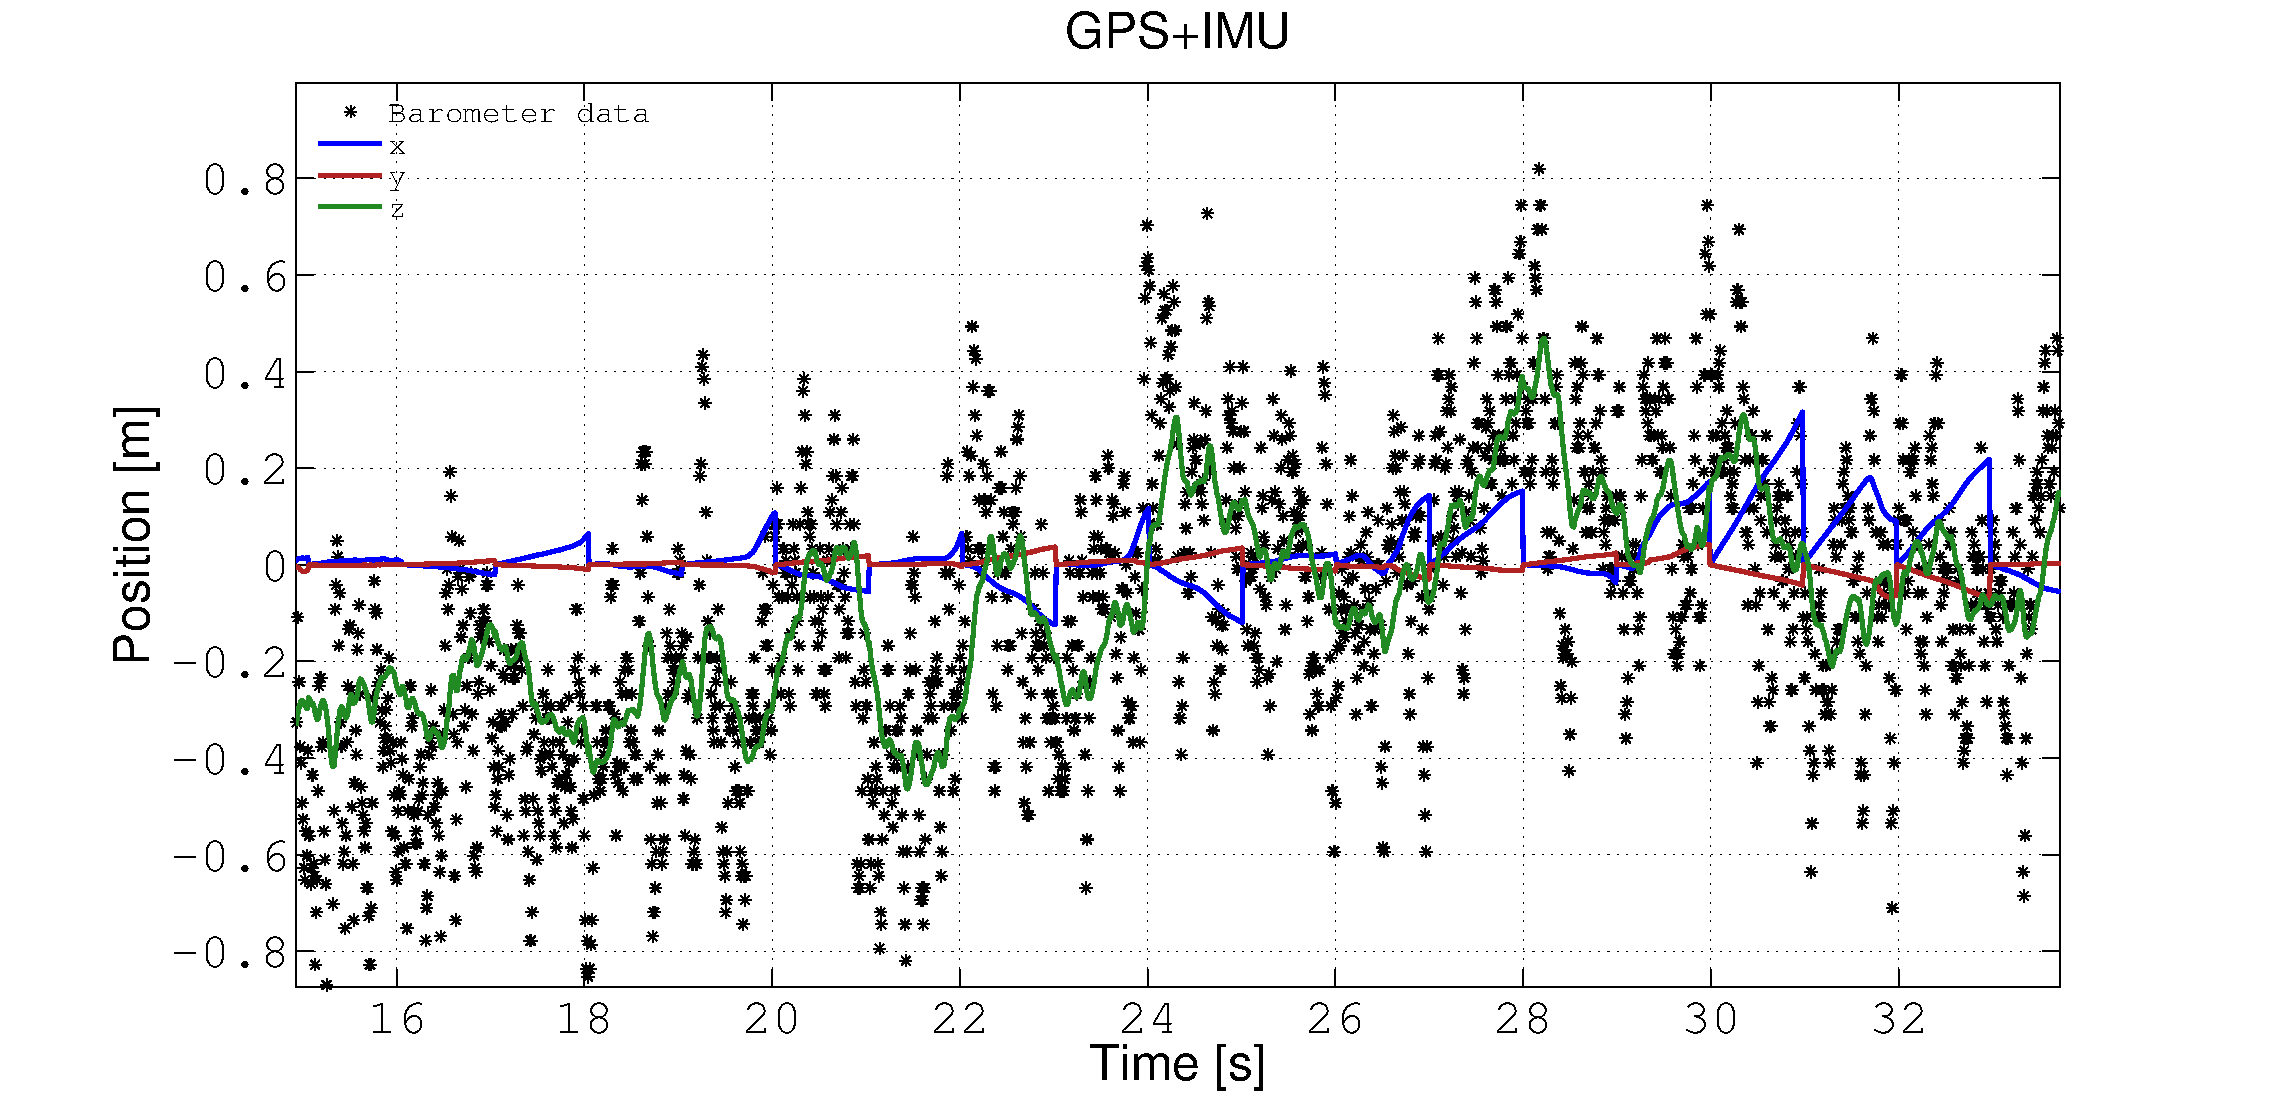
\includegraphics[width=1\columnwidth]{./pics_paper/xyz.pdf}
% 	\caption{}
% 	\label{fig:xyz.pdf}
% \end{figure}

Two different types of data will be available, depending on the availability of GPS information. When no GPS data is available there will be no direct feedback from the sensors to correct the position on the horizontal plane, only through integration, so only the prediction step can be performed for these variables.

%As shown in figure \refp{fig:xyz.pdf}, the estimation will drift until GPS data is available.

Figure \refp{fig:diagrama_kalman} shows a diagram of how data from the sensors is combined within the EKF, assisted by the model of the system. The output of the filter is an estimation the all the variables of the state vector.

\section{Control design}
\label{sec:control}

To work directly with equations \refp{eq:modelo}, a non-linear control technique would be required. To simplifly the control system, equations \refp{eq:modelo} are linearized near certain points of operation which result in a Linear Time Invariant (LTI) system of the form:
\begin{equation}
  \label{eq:lti}
  \vec{\dot{X}} = A\vec{X} + B\vec{U}
\end{equation}

This restricts the system to: Hovering\footnote{Constant state vector.}, uniform linear trajectories, and uniform circular trajectories around the vertical axis. Working with an LTI greatly simplifies the control system and does it not introduce significant limitations.

The control system is shown in figure (\refp{fig:diagrama_bloques_eng.pdf}). The feedback matrices have many entries, $K_p$ has 48 and $K_i$ has 16. A \textit{root locus} or \textit{pole-zero} analysis on such a system is not a simple task, additional complications are introduced by the fact that $K_p$ and $K_i$ will change when the trayectory changes, they depend on the linearization of the system. A simple and automated solution is achieved by means of the LQR algorithm. The initial design did not include the $K_i$ term, it was introduced to take into consideration errors in the characterization and modelling of the system.

\begin{figure}
\vspace{-60pt}
	\centering
	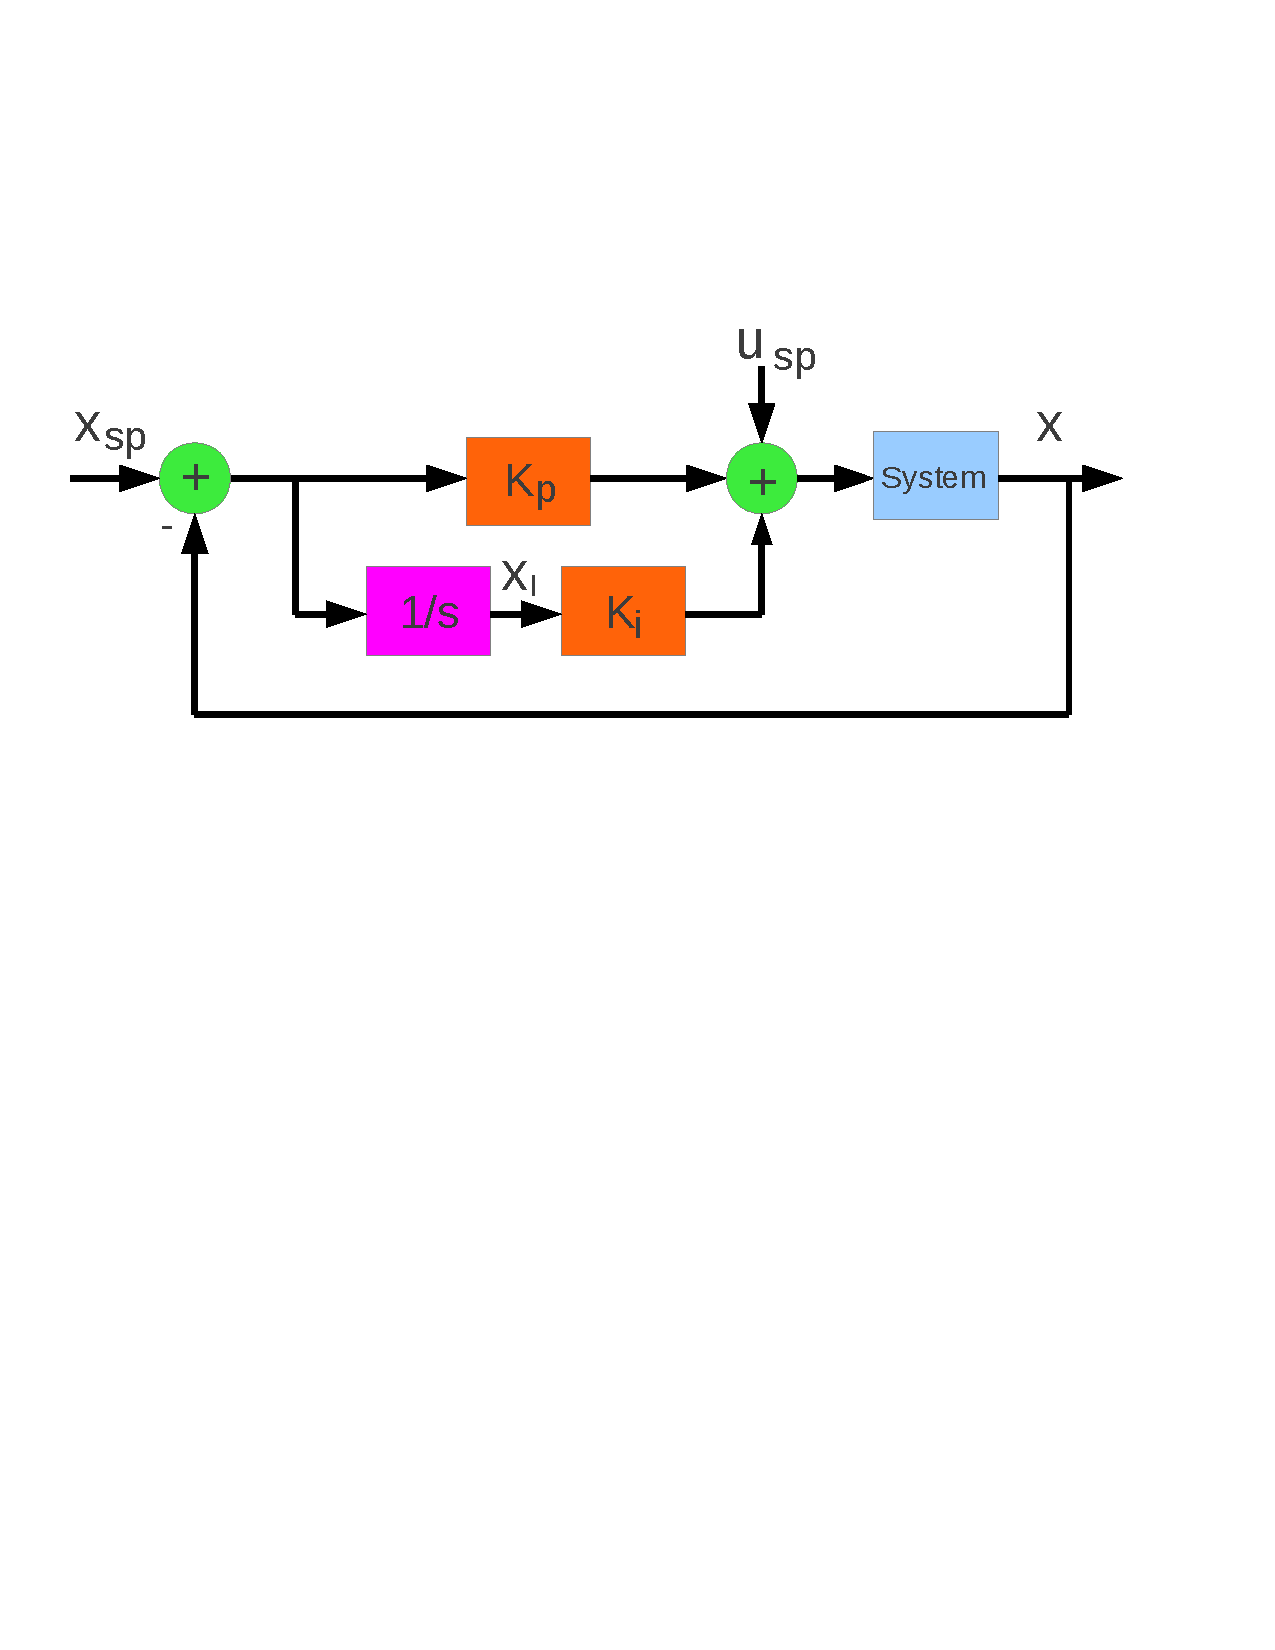
\includegraphics[width=1\columnwidth]{./pics_paper/diagrama_bloques_eng.pdf}
\vspace{-180pt}
	\caption{\textbf{Control System:} $x_{sp}$ and $u_{sp}$ represent the setpoints for the state vector and the speed of each motor. The $K_p$ and $K_i$ blocks are the proportional and integral gain matrices. The output of the system is the current state vector.}
	\label{fig:diagrama_bloques_eng.pdf}
\end{figure}

\subsection{The LQR algorithm}
\label{sec:lqr}

A a system which is controllable and observable is guaranteed to be stable and for this type of system, the LQR algorithm provides an optimal controller\cite{bib:lqrnotes} by minimizing the following cost function:

\begin{equation}
\label{eq:lqr}
\int_{0}^{\infty}  \vec{X}'(t)Q \vec{X}(t)+\vec{U}'(t)R\vec{U}(t)dt
\end{equation}

where $Q$ and $R$ are positive-definite matrices, representing the energy of the controlled states and of the control signal, respectively. The choice of $Q$ and $R$ is a tradeoff between the error that is tolerated and the energy that the system can use to correct it.

 When the system is a feedback system with known state variables, like the one shown in figure \refp{fig:diagrama_bloques_eng.pdf}, the solution is given by \refp{eq:lqr-sol}:

\begin{equation}
\begin{array}{c}
\vec{U}(t)-\vec{U}^*(t) = -K(\vec{X}(t)-\vec{X}^*(t))\\
\\
K = R^{-1}B^TP
\end{array}
\label{eq:lqr-sol}
\end{equation}

where $P$ is the solution to Riccati's equation:
\begin{equation}
  \label{eq:riccati}
  A^TP + PA - PBR^{-1}B^TP + Q = 0
\end{equation}

For the controllability and observability hypothesis to hold, only some state variables may be passed through the integral control block: $\{x,y,z,\theta\}$.

\section{Software}

\subsection{Architecture}
\label{sec:software-arch}

The software runs on several independant boards:

\begin{itemize}
\item \textbf{Flight controller:} Run by an ARM-Cortex-A8. Processes the data from the IMU, calculates the necessary control actions, and sets the desired speed for each motor by sending the appropriate commands, via $I^2C$, to the ESCs. It requires Linux specific \textit{C} functions to handle I/O. It was developed in modules, replacing any part of it should be a straightforward task. The most critical aspect of the flight controller is timing, any delays will severely degrade the performance of the system.
\item \textbf{IMU:} Uses an ATMega328p on the IMU. The firmware on the IMU takes care of reading from all the sensors (using $I^2C$) and sending a new frame of data every 10ms over a UART.
\item \textbf{ESCs:} Four microprocessors\footnote{C8051F330/1 - Silicon Labs.}, one for each motor The code running on the ESCs is not available, but the communication protocol was decoded using a logic analyzer.
\end{itemize}

The flight controller is accesed via an \textit{ssh} session over \textit{WiFi}. Once logged in, the flight controller software can be compiled and executed.

\subsection{Implementation details}
\label{sec:software-impl}

The code implements a discrete version of the LQR control system mentioned in \refp{sec:control}, based on a discretization of the model described in \refp{sec:modelo}. There are some practical considerations worth mentioning:
\begin{itemize}
\item \textbf{Saturation:} The integral term saturates it is designed to compensate for small errors in characterization/modelling and should never grow too much. Large diferences between the current state and the setpoint should be handled by the proportional term.
\item \textbf{Limiting:} The control block sets $\vert \vec{X} - \vec{X}_{sp}\vert < \vert \vec{X}_{th} \vert$ to avoid attempts to perform actions that the system cannot handle.
\end{itemize}


\section{Results}

\subsection{Tests}
\label{sec:results-tests}

The testing phase was separated into several parts:

\begin{enumerate}
\item \textbf{Basic Stability}: During this first stage, the quadcopter was only allowed to move (and correct) one of the Euler angles $\{\psi,\phi\}$. The control system was tuned until an acceptable behavior was obtained. This procedure was applied to each angle. Once this stage was completed the quadcopter was able to mantain horizontality by controlling $\{\psi,\phi,\omega_{q_x},\omega_{q_y}\}$.
\item \textbf{Orientation}: To verify orientation was correctly maintained the speed of the motors was reduced, below the level required to lift off, and the quadcopter was hung from strings. During this test offsets can be set on each motors to compensate for differences between them. After this test, the control system was able to hold the last of the Euler angles: $\{\theta,\omega_{q_z}\}$.
\item \textbf{Limited flying}: At this point the three Euler angles are controlled, so a basic level of stability is expected. During this stage strings were attached to the quadcopter from the top and bottom, and it was allowed to fly. After this test, the control system was able to take-off and to hold altitud and vertical speed: $\{z,v_{q_z}\}$.
\item \textbf{Free flight}: The last step was to let the quadcopter fly. This stage required the GPS. After it was completed, the control system was able to hold it's horizontal position $\{x,y,v_{q_x},v_{q_y}\}$, completing control over the state variables.
\end{enumerate}

Free flight tests were limited due to the poor reliabitily of the ESCs provided by LotusRC\footnote{\url{http://www.lotusrc.com/}}, which showed issues such as overheating until burning out and random glitches that would cause motors to turn off.

\subsection{System response}
\label{sec:results-system-response}

To ilustrate some results, figure \refp{fig:psi_esc.pdf} shows the step response for $\psi$ during an experiment where this was the only degree of freedom. Figure \refp{fig:altura.pdf} shows altitud during takeoff from altitud 0m until a target altitud of 1m.

\begin{figure}
	\centering
	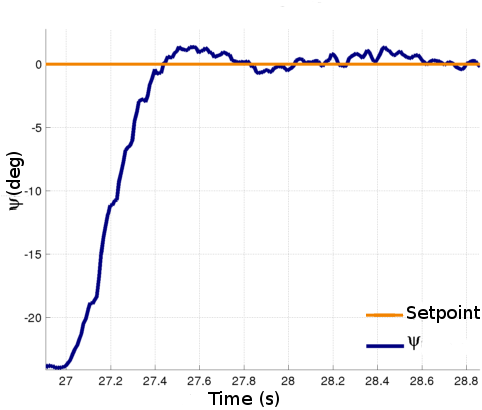
\includegraphics[width=.9\columnwidth]{./pics_paper/control_escalon_eng.png}
	\caption{\textbf{Step response:} Performance during an experiment limited to a single degree of freedom ($\psi$).}
	\label{fig:psi_esc.pdf}
\end{figure}

\begin{figure}
	\centering
	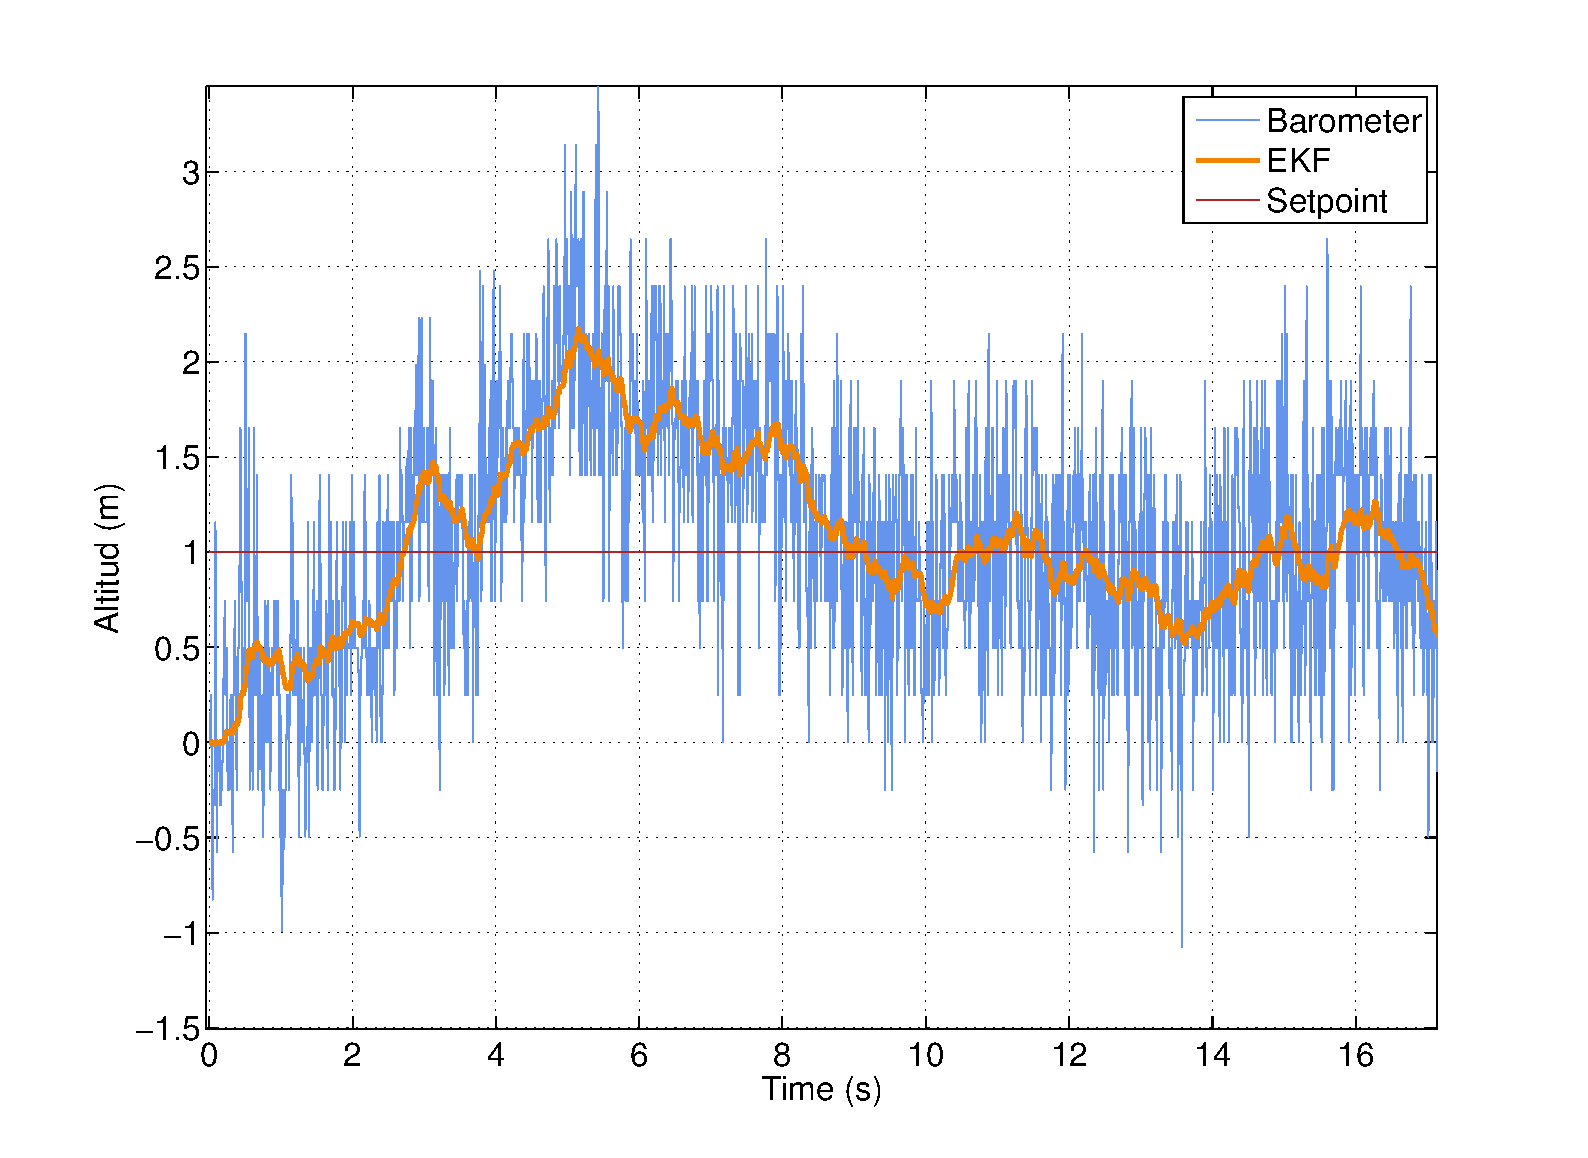
\includegraphics[width=1\columnwidth]{./pics_paper/altura.pdf}
	\caption{\textbf{Altitud:} Performance during takeoff (from 0m to 1m).}
	\label{fig:altura.pdf}
\end{figure}

Flight test were satisfactory in windless environments. In presence of wind the system is not stable. The aluminium protections added (to protect the motors from the faulty ESCs) have flat surfaces that may intensify the effect of the wind.

% An example of a floating figure using the graphicx package.
% Note that \label must occur AFTER (or within) \caption.
% For figures, \caption should occur after the \includegraphics.
% Note that IEEEtran v1.7 and later has special internal code that
% is designed to preserve the operation of \label within \caption
% even when the captionsoff option is in effect. However, because
% of issues like this, it may be the safest practice to put all your
% \label just after \caption rather than within \caption{}.
%
% Reminder: the "draftcls" or "draftclsnofoot", not "draft", class
% option should be used if it is desired that the figures are to be
% displayed while in draft mode.
%
%\begin{figure}[!t]
%\centering
%\includegraphics[width=2.5in]{myfigure}
% where an .eps filename suffix will be assumed under latex, 
% and a .pdf suffix will be assumed for pdflatex; or what has been declared
% via \DeclareGraphicsExtensions.
%\caption{Simulation Results}
%\label{fig_sim}
%\end{figure}

% Note that IEEE typically puts floats only at the top, even when this
% results in a large percentage of a column being occupied by floats.


% An example of a double column floating figure using two subfigures.
% (The subfig.sty package must be loaded for this to work.)
% The subfigure \label commands are set within each subfloat command, the
% \label for the overall figure must come after \caption.
% \hfil must be used as a separator to get equal spacing.
% The subfigure.sty package works much the same way, except \subfigure is
% used instead of \subfloat.
%
%\begin{figure*}[!t]
%\centerline{\subfloat[Case I]\includegraphics[width=2.5in]{subfigcase1}%
%\label{fig_first_case}}
%\hfil
%\subfloat[Case II]{\includegraphics[width=2.5in]{subfigcase2}%
%\label{fig_second_case}}}
%\caption{Simulation results}
%\label{fig_sim}
%\end{figure*}
%
% Note that often IEEE papers with subfigures do not employ subfigure
% captions (using the optional argument to \subfloat), but instead will
% reference/describe all of them (a), (b), etc., within the main caption.


% An example of a floating table. Note that, for IEEE style tables, the 
% \caption command should come BEFORE the table. Table text will default to
% \footnotesize as IEEE normally uses this smaller font for tables.
% The \label must come after \caption as always.
%
%\begin{table}[!t]
%% increase table row spacing, adjust to taste
%\renewcommand{\arraystretch}{1.3}
% if using array.sty, it might be a good idea to tweak the value of
% \extrarowheight as needed to properly center the text within the cells
%\caption{An Example of a Table}
%\label{table_example}
%\centering
%% Some packages, such as MDW tools, offer better commands for making tables
%% than the plain LaTeX2e tabular which is used here.
%\begin{tabular}{|c||c|}
%\hline
%One & Two\\
%\hline
%Three & Four\\
%\hline
%\end{tabular}
%\end{table}


% Note that IEEE does not put floats in the very first column - or typically
% anywhere on the first page for that matter. Also, in-text middle ("here")
% positioning is not used. Most IEEE journals/conferences use top floats
% exclusively. Note that, LaTeX2e, unlike IEEE journals/conferences, places
% footnotes above bottom floats. This can be corrected via the \fnbelowfloat
% command of the stfloats package.



\section{Conclusion}

The main goal of the project was achieved: A quadcopter able to fly on its own. The system was successfully tested. A basic control was implemented, capable of stabilizing the system. The doors are open for future projects to add additional levels of intelligence allowing the quadcopter to perform tasks such as power line inspection, surveillance, assitance during natural disasters, etc.

\subsection{Future Work}
\begin{itemize}
\item The LotusRC ESCs proved to be extremely unreliable\footnote{Several versions were tested, all of then showed the same issues.} and severly delayed the project. Replacing the ESCs is a critical task.
\item The choice of implementing the flight controller on an operating system that does not run in real-time made timing a complicated issue. These issues were dealt with, but assinging additional tasks to the system will surely distrupt timing. Porting the stabilization system, which requires a very fast and steady loop, to a dedicated microprocessor would be a significant improvement. It would allow the code running on top of the operating system to perform higher level tasks, such as Visual Simultaneous Localization and Mapping (VSLAM), navigation, tracking, etc.
\item The fact that the system does not work in a windy environment severly limits the range of possible applications, solving this issue by either reducing the aerodynamic resistance or implementing a different control system would be a significant improvement.
%TODO paper q dijo el pater del viento.
\end{itemize}

% conference papers do not normally have an appendix


% use section* for acknowledgement
\section*{Acknowledgment}

The authors would like to thank family and friends for their support during this year, and the staff of the University for their commitment to the project.

% trigger a \newpage just before the given reference
% number - used to balance the columns on the last page
% adjust value as needed - may need to be readjusted if
% the document is modified later
%\IEEEtriggeratref{8}
% The "triggered" command can be changed if desired:
%\IEEEtriggercmd{\enlargethispage{-5in}}

% references section

% can use a bibliography generated by BibTeX as a .bbl file
% BibTeX documentation can be easily obtained at:
% http://www.ctan.org/tex-archive/biblio/bibtex/contrib/doc/
% The IEEEtran BibTeX style support page is at:
% http://www.michaelshell.org/tex/ieeetran/bibtex/
%\bibliographystyle{IEEEtran}
% argument is your BibTeX string definitions and bibliography database(s)
%\bibliography{IEEEabrv,../bib/paper}
%
% <OR> manually copy in the resultant .bbl file
% set second argument of \begin to the number of references
% (used to reserve space for the reference number labels box)
\bibliographystyle{ieeetr} 
\bibliography{../biblio}
% \begin{thebibliography}{1}

% \bibitem{IEEEhowto:kopka}
% H.~Kopka and P.~W. Daly, \emph{A Guide to \LaTeX}, 3rd~ed.\hskip 1em plus
%   0.5em minus 0.4em\relax Harlow, England: Addison-Wesley, 1999.
% \end{thebibliography}

% that's all folks
\end{document}


